% Chapter 4

\chapter{Methods for determination of other parameters of MOS structure.}\label{Chapter4}
\lhead{Chapter 4. \emph{Methods for determination of other parameters of MOS structure}}
%- - - - - - - - - - - - - - - - - - - - - - - - - - - - - - - - - - - - - - - - - - - -

In Chapter~\ref{Chapter3} we have described the C-V methods that we
will use to determine the parameters of MOS\@ structures. In
particular, we we will deal with the determination of the
concentration profile of the donating impurities in the subsurface
region of the semiconductor, since some methods of determining other
MOS structure parameters are based on the assumption that the
concentration is known. In determining the concentration profile
curves, which are not homogeneous, models are used whose accuracy
of approximating a given physical phenomenon depends on the
concentration gradient admixture~\cite{4.1, 4.2, 4.3, 4.4}. In order
to verify the accuracy of the used approximations, we performed a
comparison of the concentration profiles:

\begin{itemize}
\item used in the calculation of the theoretical C-V dependence and
\item obtained from this theoretical C-V dependence~\cite{4.5}.
\end{itemize}

The results are given in Section~\ref{sec:4.1.4}.

\par The next parameter we will determine is the density of traps
of the $Si-SiO_{2}$ interface. Here, two
procedures. Comparison of high and low frequency C-V
dependence, or a comparison of experimental and theoretical C-V
dependence. Their application is described in Section~\ref{sec:4.2}.

\par Determination of the generation lifetime of minority charge carriers that
related to the constant-width SCR method, has been described in Section~\ref{sec:3.4}.

\section[Determination of the concentration profile of impurities]{Determination of the concentration profile of impurities in the subsurface region of the semiconductor.}\label{sec:4.1}

The subject of measuring concentration profiles was addressed in our
department in the paper~\cite{4.6}. Here we will address only some
aspects of this subject that are related to the determination of
inhomogeneous concentration profile of dopants in a semiconductor.

\par Separate areas of concern in determining the concentration
profile of impurities, which we denote by $N(x)$, consist of:

\begin{itemize}
\item correction of the calculated concentration in the region from
  the surface of the semiconductor to a depth of $2L_{DE}$~\cite{4.7,
    4.8}
\item determination of the depth of the calculated concentration,
  relying on models determining the width of the SCR~\cite{4.9, 4.10,
    4.11}
\item correction for the effect of $Si-SiO_2$ interface
  traps~\cite{4.12}
\item the difference between the concentration of the interfering
  impurities $N(x)$ and the concentration of the majority charge
  carriers $n(x)$.
\end{itemize}

\subsection[Correction of the concentration of interfering impurities]{Correction of the concentration of interfering impurities at the surface of the semiconductor.}\label{sec:4.1.1}

Known equation for calculating $N(x)$~\cite{I.2}

\begin{equation}\label{eq:4.1}
  N(x) = {\frac{2}{q\epsilon}} {\Bigg[\frac{dC_{sc}^{-2}}{d\varphi_{s}}\Bigg]}^{-1}
\end{equation}

was derived from the solution of the Poisson equation using the
approximation of deep depletion. This approximation does not hold for
SCR widths smaller than $2L_{DE}$. In order to obtain correct results
also in this region, we need to correct $N(x)$ computed according
to~\ref{eq:4.1} by the procedure derived in~\cite{4.7, 4.8}.  The
correction is a function of the surface potential. Its physical
significance is evident from the work~\cite{4.7}.

\begin{equation}\label{eq:4.2}
  {N(x)}_{corrected} = N(x)f(\varphi_{s})
\end{equation}

, where

\begin{equation}\label{eq:4.3}
  f(\varphi_{s}) = {\frac{1}{1-e^{-\beta\varphi_{s}}}} - {\frac{2e^{-\beta\varphi_{s}}\big[e^{-\beta\varphi_{s}}+\beta\varphi_{s} -1\big]}{\big[1-e^{-\beta\varphi_{s}}\big]}} \qquad, where\quad \beta=\frac{q}{kT}
\end{equation}

The surface potential used in equation~\ref{eq:4.3} can be determined
according to~\cite{4.7} by numerically solving the equation

\begin{equation}\label{eq:4.4}
  \frac{C_{sc}^{2}}{\varphi_{s}}\frac{C_{sc}^{-2}}{d\varphi_{s}}=\frac{1-e^{-\beta\varphi_{s}}}{e^{-\beta\varphi_{s}}+\beta\varphi_{s}-1}-\frac{2e^{-\beta\varphi_{s}}} {1-e^{-\beta\varphi_{s}}}
\end{equation}

It should be noted here that the equation~\ref{eq:4.4} was derived
using the relation for the SCR capacity $C_{sc}$, which assumes a
homogeneous concentration of dopants. Since the experimentally
determined differential capacitance $C_{sc}$ depends on the change in
charge at the SCR boundary (which uses equation~\ref{eq:4.1}), the
surface potential obtained from equation~\ref{eq:4.4} will represent
the potential that would be at the surface of the semiconductor if the
concentration of $N(x)$ across the SCR region were constant and also
equal to the concentration at the SCR boundary (which we determine
according to~\ref{eq:4.1}). It follows that for inhomogeneously doped
substrates the equation~\ref{eq:4.4} cannot be used to obtain the true
values of $\varphi_{s}(V_{g})$, despite the fact that the
correction~\ref{eq:4.2} gives good results in this case as well.

\subsection[Determination of the depth of the concentration profile.]{Determination of the depth of the concentration profile.}\label{sec:4.1.2}

Having determined the concentration according to the
equation~\ref{eq:4.2}, it is also necessary to determine the location
of the calculated concentration. A commonly used relationship based on
plate capacitor model (which is an approximation of the deep
depletion)

\begin{equation}\label{eq:4.5}
  w(C_{sc})=\frac{\epsilon}{C_{sc}}
\end{equation}

is not valid for depths less than $2L_{DE}$. In this region, it is
possible to use the relation derived using an approximation of the
curve of the electric potential in semiconductor $\varphi(x)$. The
above problem has been discussed in detail in our department
in~\cite{4.13, 4.14}, where the results of work~\cite{4.9, 4.10, 4.11}
were used. To calculate the depth in this region, we can use a
relation that is an approximation of the curve of the electric
potential in semiconductor $\varphi(x)$~\cite{I.1}

\begin{equation}\label{eq:4.6}
  w(\varphi_{s})=\sqrt{2}L_{DE}{\big[e^{-\beta\varphi_{s}}+\beta\varphi_{s}-1\big]}^{\frac{1}{2}}
\end{equation}

, where

\begin{equation}\label{eq:4.7}
  L_{DE} = {\Big[\frac{\epsilon}{\beta qN}\Big]}^{\frac{1}{2}}
\end{equation}

is the extrinsic Debay length, which we used in the calculation the
concentration obtained from the equation~\ref{eq:4.2}.  In
equation~\ref{eq:4.6} we use the value of $\varphi_{s}$ obtained from
the solution equation~\ref{eq:4.4}. Despite the fact that also the
equation~\ref{eq:4.6} was derived assuming a homogeneous distribution
of impurities in the semiconductor, its use in conjunction with the
solution of equation~\ref{eq:4.4} gives a satisfactory results, as we
shall show later.

\begin{figure}[h!]\centering
  \begin{minipage}[c]{\myfiguresize}
    \begin{center}
      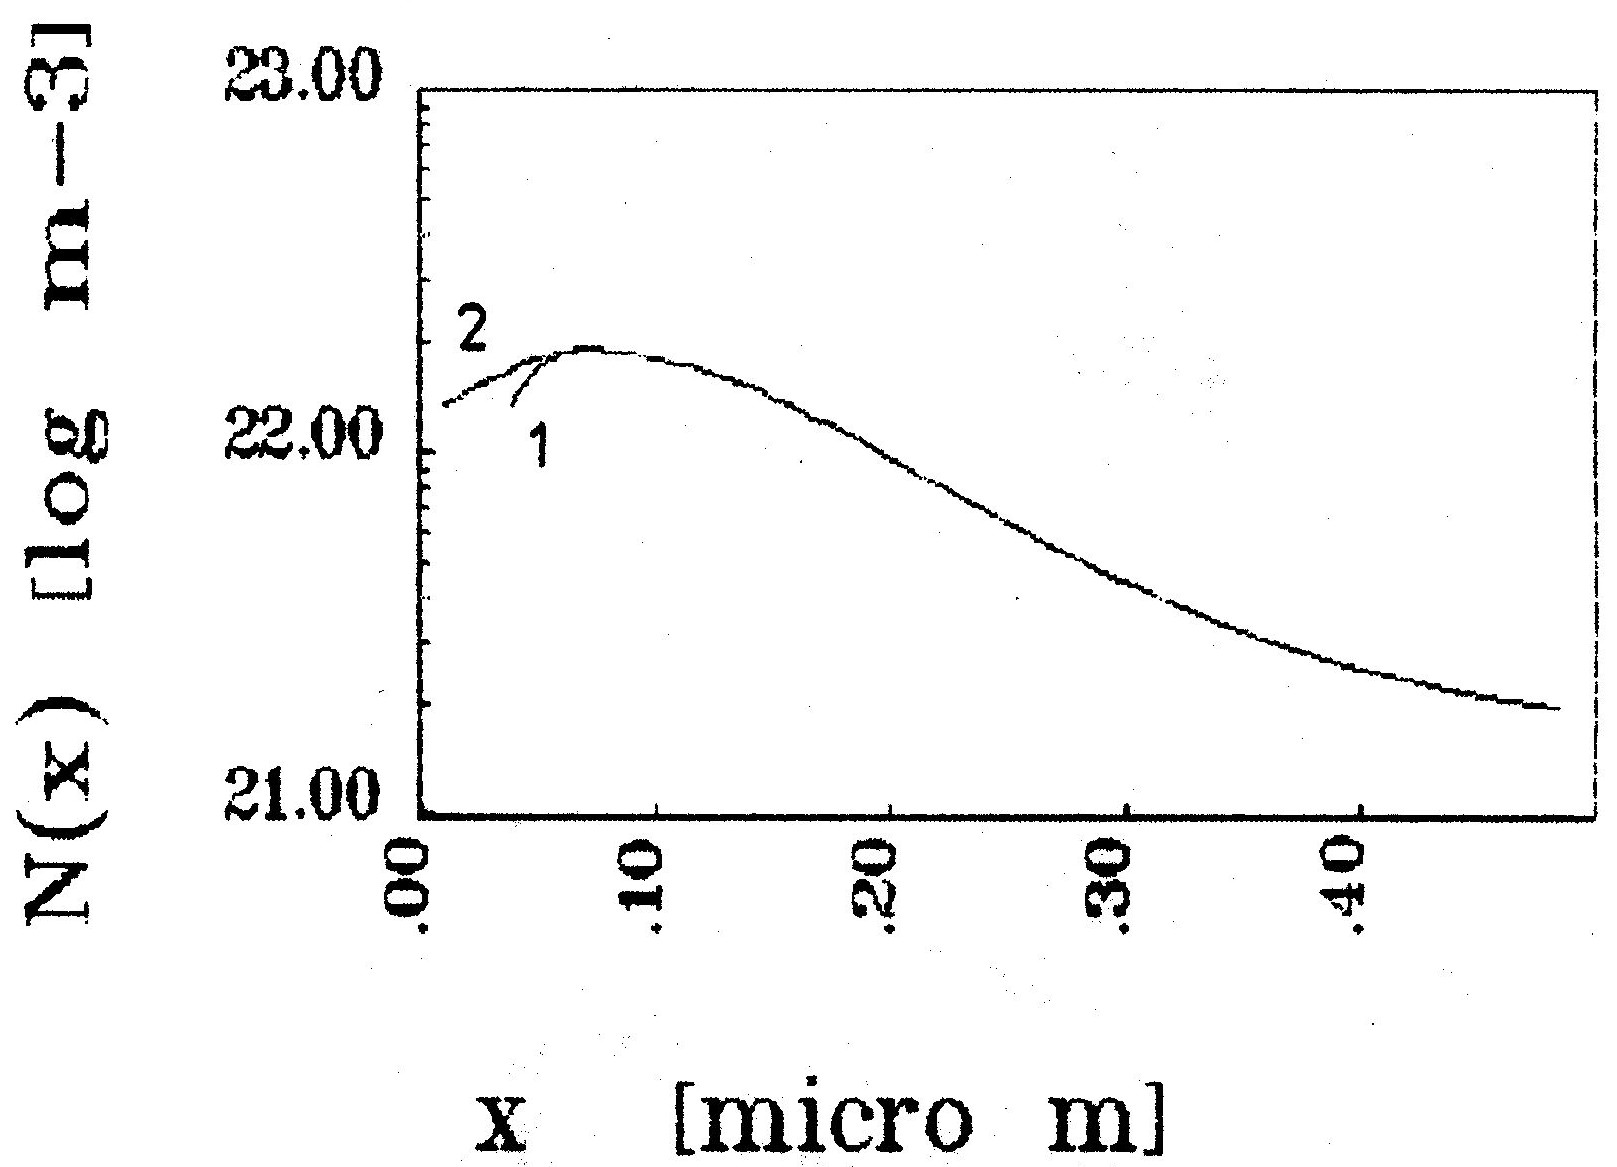
\includegraphics{Figures/fig-4-1.eps}% chktex-file 8
      \caption[Concentration profile of dopants in a semiconductor
        calculated from the equation~\ref{eq:4.2}]{Concentration
        profile of the dopants in the semiconductor calculated from
        the equation~\ref{eq:4.2}. The distance from the surface was
        determined from the equation~\ref{eq:4.5} (curve 1)
        and~\ref{eq:4.6} (curve 2).}\label{fig:4.1}
    \end{center}
  \end{minipage}
\end{figure}
% OBR26.BIT

Figure~\ref{fig:4.1} shows the curves of $N(x)$ using
correction~\ref{eq:4.2}, presenting the difference in using
equations~\ref{eq:4.5} and~\ref{eq:4.6}. Here it is clear that by
using equation~\ref{eq:4.6} one can calculate the path of the
concentration of the dopants closer to the semiconductor surface.
This is of importance for further calculations, which presuppose
knowledge of the $N(x)$ curve.

The first column of the table~\ref{tab:4.1} contains the values of
$\varphi_{s}$ determined by solving the equation~\ref{eq:4.4} and the
second column contains the values of the correction
factor~\ref{eq:4.3}. The other two columns allow comparison of the
uncorrected and corrected values of $N(x)$ and the last two columns
give the values of $w(\varphi_{s})$ and $w(C_{sc})$ obtained from the
equations~\ref{eq:4.5} and~\ref{eq:4.6}.

\begin{table}[h!]\centering
  \begin{minipage}[c]{\myfiguresize}
    \begin{center}
      \begin{tabular}{c c c c c c c c c c}
        $\varphi_{s}[V]$ & $f(\varphi_{s})$ & $N[m^{-3}]$ & $N_{cor.}[m^{-3}]$ & $w(\varphi_{s})[\mu m]$ & $w(C_{SC})[\mu m]$ \\
        \hline% chktex-file 44
        0.007 & 0.39 & $0.35\times10^{23}$ & $0.14\times10^{23}$ & 0.0102 & 0.0389 \\
        0.016 & 0.44 & $0.33\times10^{23}$ & $0.15\times10^{23}$ & 0.0190 & 0.0413 \\
        0.024 & 0.50 & $0.31\times10^{23}$ & $0.15\times10^{23}$ & 0.0265 & 0.0438 \\
        0.032 & 0.56 & $0.29\times10^{23}$ & $0.16\times10^{23}$ & 0.0333 & 0.0466 \\
        0.041 & 0.61 & $0.28\times10^{23}$ & $0.17\times10^{23}$ & 0.0391 & 0.0494 \\
        0.049 & 0.66 & $0.27\times10^{23}$ & $0.18\times10^{23}$ & 0.0444 & 0.0523 \\
        0.057 & 0.71 & $0.26\times10^{23}$ & $0.18\times10^{23}$ & 0.0493 & 0.0553 \\
        0.065 & 0.76 & $0.25\times10^{23}$ & $0.19\times10^{23}$ & 0.0538 & 0.0585 \\
        0.073 & 0.80 & $0.24\times10^{23}$ & $0.19\times10^{23}$ & 0.0581 & 0.0617 \\
        0.081 & 0.83 & $0.23\times10^{23}$ & $0.19\times10^{23}$ & 0.0623 & 0.0650 \\
        0.090 & 0.86 & $0.22\times10^{23}$ & $0.19\times10^{23}$ & 0.0664 & 0.0684 \\
        0.098 & 0.89 & $0.22\times10^{23}$ & $0.19\times10^{23}$ & 0.0704 & 0.0719 \\
        0.106 & 0.91 & $0.21\times10^{23}$ & $0.19\times10^{23}$ & 0.0743 & 0.0755 \\
        0.115 & 0.93 & $0.21\times10^{23}$ & $0.19\times10^{23}$ & 0.0783 & 0.0791 \\
        0.124 & 0.94 & $0.20\times10^{23}$ & $0.19\times10^{23}$ & 0.0822 & 0.0828 \\
        0.133 & 0.96 & $0.20\times10^{23}$ & $0.19\times10^{23}$ & 0.0861 & 0.0866 \\
        0.142 & 0.97 & $0.19\times10^{23}$ & $0.19\times10^{23}$ & 0.0900 & 0.0904 \\
        0.151 & 0.97 & $0.19\times10^{23}$ & $0.18\times10^{23}$ & 0.0939 & 0.0942 \\
        0.160 & 0.98 & $0.19\times10^{23}$ & $0.18\times10^{23}$ & 0.0978 & 0.0981 \\
        0.169 & 0.99 & $0.18\times10^{23}$ & $0.18\times10^{23}$ & 0.1018 & 0.1019 \\
        0.178 & 0.99 & $0.18\times10^{23}$ & $0.18\times10^{23}$ & 0.1058 & 0.1058 \\
        0.187 & 0.99 & $0.18\times10^{23}$ & $0.17\times10^{23}$ & 0.1098 & 0.1098 \\
        0.205 & 1.00 & $0.17\times10^{23}$ & $0.17\times10^{23}$ & 0.1179 & 0.1179 \\
      \end{tabular}
      \caption[Calculation of dopant concentration profile
        $N(x)$]{Calculation of dopant concentration profile
        $N(x)$.}\label{tab:4.1}
    \end{center}
  \end{minipage}
\end{table}

\begin{minipage}[c]{\textwidth}
  \emph{NOTE.} Using the approximation~\ref{eq:4.6}, which represents
  the width of the SCR as as a function of the surface potential of
  the semiconductor (the concentration is parameter), one can
  approximate the path of $\varphi(x)$ for a given SCR width even if
  the semiconductor substrate is inhomogeneously doped.  Custom
  procedure for determining the concentration of dopant impurities
  from capacitance measurements is a discretization of the continuous
  $N(x)$ curve, where the individual values of $N_i$ represent an
  approximation of the concentration in the region of the boundary
  SCR~\cite{4.1, 4.2, 4.3}.  The loss of the potential
  $\Delta\varphi_i$ at layer of width $\Delta w_{i}=w_{i+1}-w_{i}$
  with concentration $N_i$ can be determined by solving the equation
  \begin{equation}\label{eq:4.8}
    \Delta w_{i} = \sqrt{2}L_{DE_{i}}{\Big[e^{-\beta\Delta\varphi_{i}} + \beta\Delta\varphi_{i} - 1\Big]}^{\frac{1}{2}}
  \end{equation}
  , where% chktex-file 26
  \begin{equation}\label{eq:4.9}
    L_{DE_{i}} = {\bigg[\frac{\epsilon}{\beta qN_{i}}\bigg]}^{\frac{1}{2}}
  \end{equation}
  Then the progression of $\varphi(x)$ can be obtained using the
  equations~\ref{eq:4.8} and~\ref{eq:4.9} if we start the calculation
  from the SCR boundary, where we assume potential is zero, towards
  the surface of the semiconductor.
\end{minipage}

\subsection[Effect of $Si-SiO_{2}$ interface traps and minority charge carrier generation]{Effect of $Si-SiO_{2}$ interface traps and minority charge carrier generation}\label{sec:4.1.3}

Minority carrier generation occurs in the inversion region of the SCR
charge generation, which forms the inversion layer and affects the
magnitude of the capacitance of the MOS\@ structure. In order to
measure the C-V dependence in the deep depletion that is not affected
by minority charge carriers, we will use the pulsed HF C-V method. The
measured values of $N(x)$ obtained using this method are shown in
Figure~\ref{fig:4.2}.

\begin{figure}[h!]\centering
  \begin{minipage}[c]{\myfiguresize}
    \begin{center}
      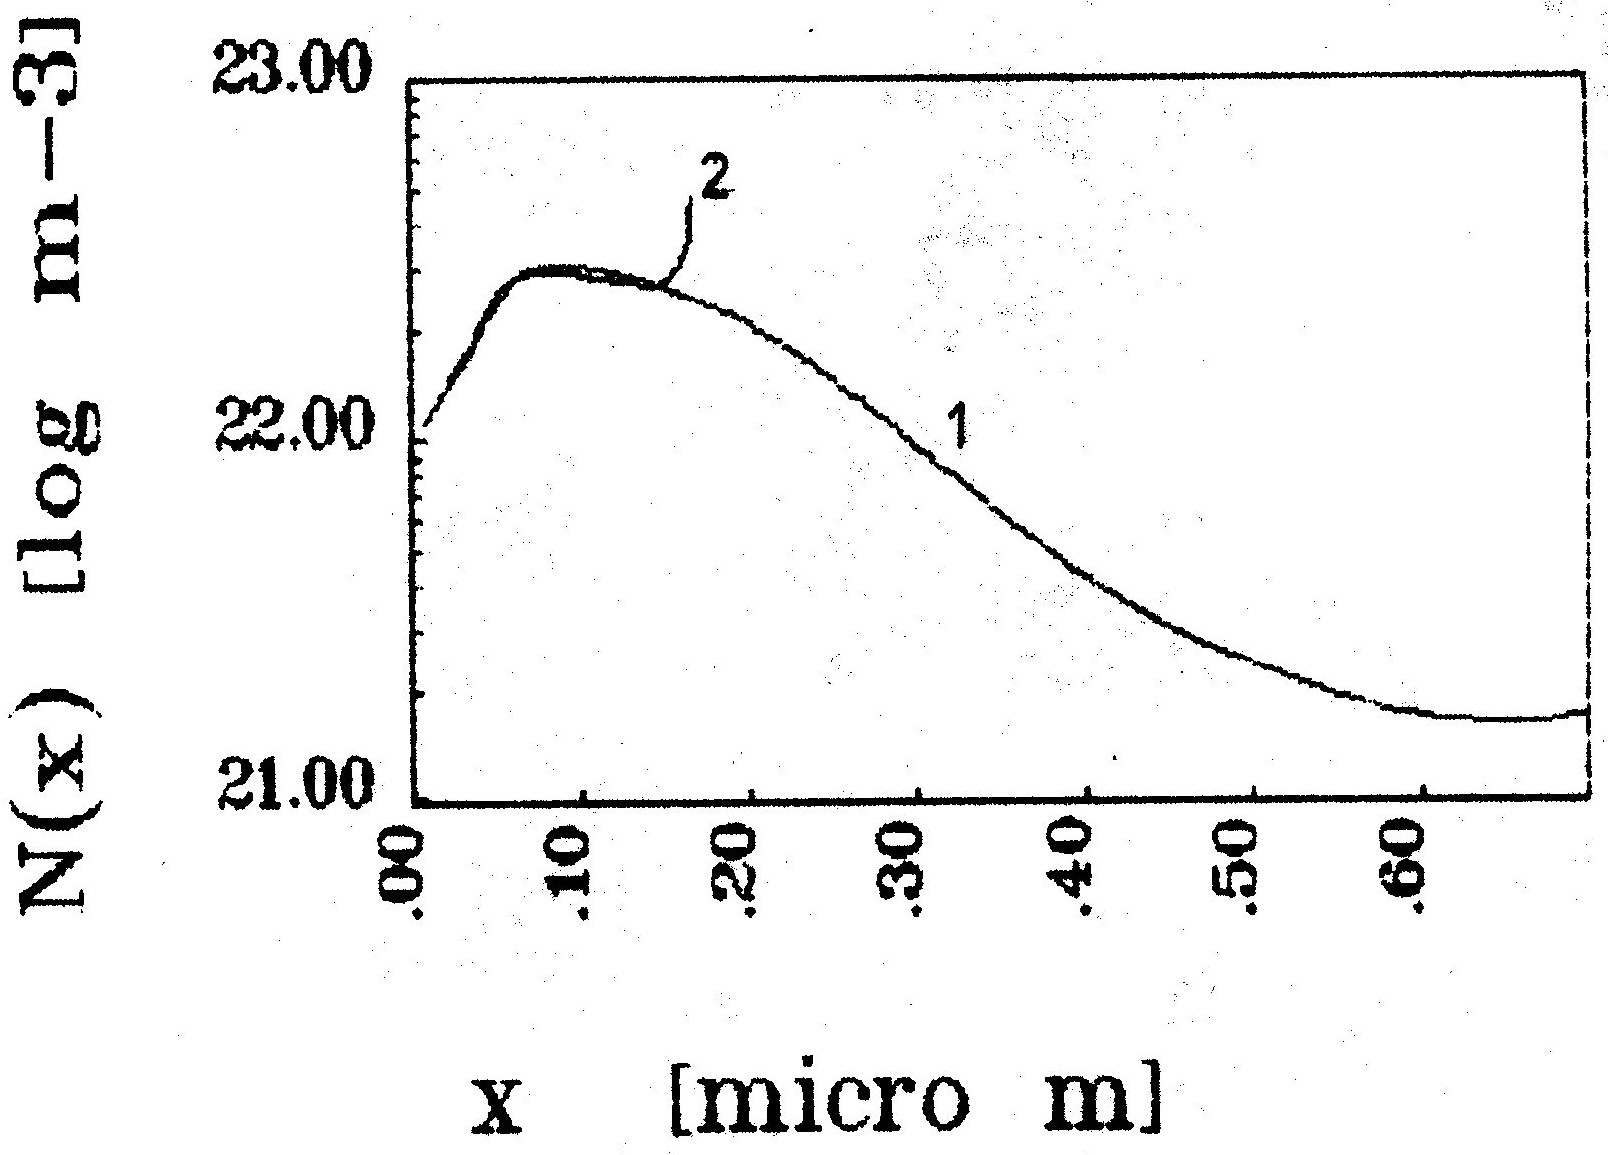
\includegraphics{Figures/fig-4-2.eps}% chktex-file 8
      \caption[Concentration profile of interfering impurities
        obtained from C-V dependence in the deep depletion region and
        from the equilibrium C-V dependence]{Current concentration
        profile of the interfering impurities obtained from the C-V
        dependence in the deep depletion region (curve 1) and from the
        equilibrium C-V dependence (curve 2). To calculate $N(x)$
        dependence, the C-V dependences shown in
        Figure~\ref{fig:3.2}}\label{fig:4.2}
    \end{center}
  \end{minipage}
\end{figure}
% OBR8.BIT

\par When calculating $N(x)$ using
equations~\ref{eq:4.1},~\ref{eq:4.2},~\ref{eq:4.3},~\ref{eq:4.4}
and~\ref{eq:4.6} the approximation is used

\begin{equation}\label{eq:4.10}
  \frac{dC_{sc}^{-2}}{d\varphi_{s}} \cong \frac{dC_{mos}^{-2}}{dV_{g}}
\end{equation}

where equality holds if the trap density of the $Si-SiO_{2}$ interface
is zero. However, the measured HF C-V dependence is always to some
extent affected by the interface traps, which change their
state~\cite{4.15}. This influence can be reduced by increasing the
frequency of the measurement signal and by measuring the capacitance
faster after the voltage jump pulsed C-V method.  The problem of using
the approximation~\ref{eq:4.10} is avoided if we use the data measured
by Q-C to determine $N(x)$ method, where we can determine the surface
potential curve $\varphi_{s}(V_{g})$. If we determine the
concentration profile of the dopants from the HF C-V dependence, we
can correct for the effect of the $Si-SiO_{2}$ interface traps in
depletion region by the relation given in~\cite{I.1}

\begin{equation}\label{eq:4.11}
  {N(x)}_{corrected} = {N(x)}{\cfrac{1-\cfrac{C_{mos}^{LF}}{C_{ox}}}{1-\cfrac{C_{mos}^{HF}}{C_{ox}}}}
\end{equation}

assuming we know the low-frequency C-V dependence.

\subsection[Calculation of the concentration profile of impurities from the curve of major charge carriers.]{Calculation of the concentration profile of impurities from the curve of major charge carriers.}\label{sec:4.1.4}

As can be seen from Figure~\ref{fig:1.1}, for the inhomogeneous
curve of the concentration of the donor atoms occurs due to
diffusion of the majority charge carriers, there is a difference
between the above curves~\cite{4.16}. It known~\cite{4.17} that by
using the equation~\ref{eq:4.1} we determine the curve of the
concentration of the majority charge carriers instead of the
concentration of the contaminating impurities. A correction is
described in the work of~\cite{4.18}, using the which can be used to
determine the exact concentration of the interfering atoms from the
measured $n (x)$ (if the measured $n (x)$ actually represents the
curve of the major charge carriers).

\begin{figure}[h!]\centering
  \begin{minipage}[c]{\myfiguresize}
    \begin{center}
      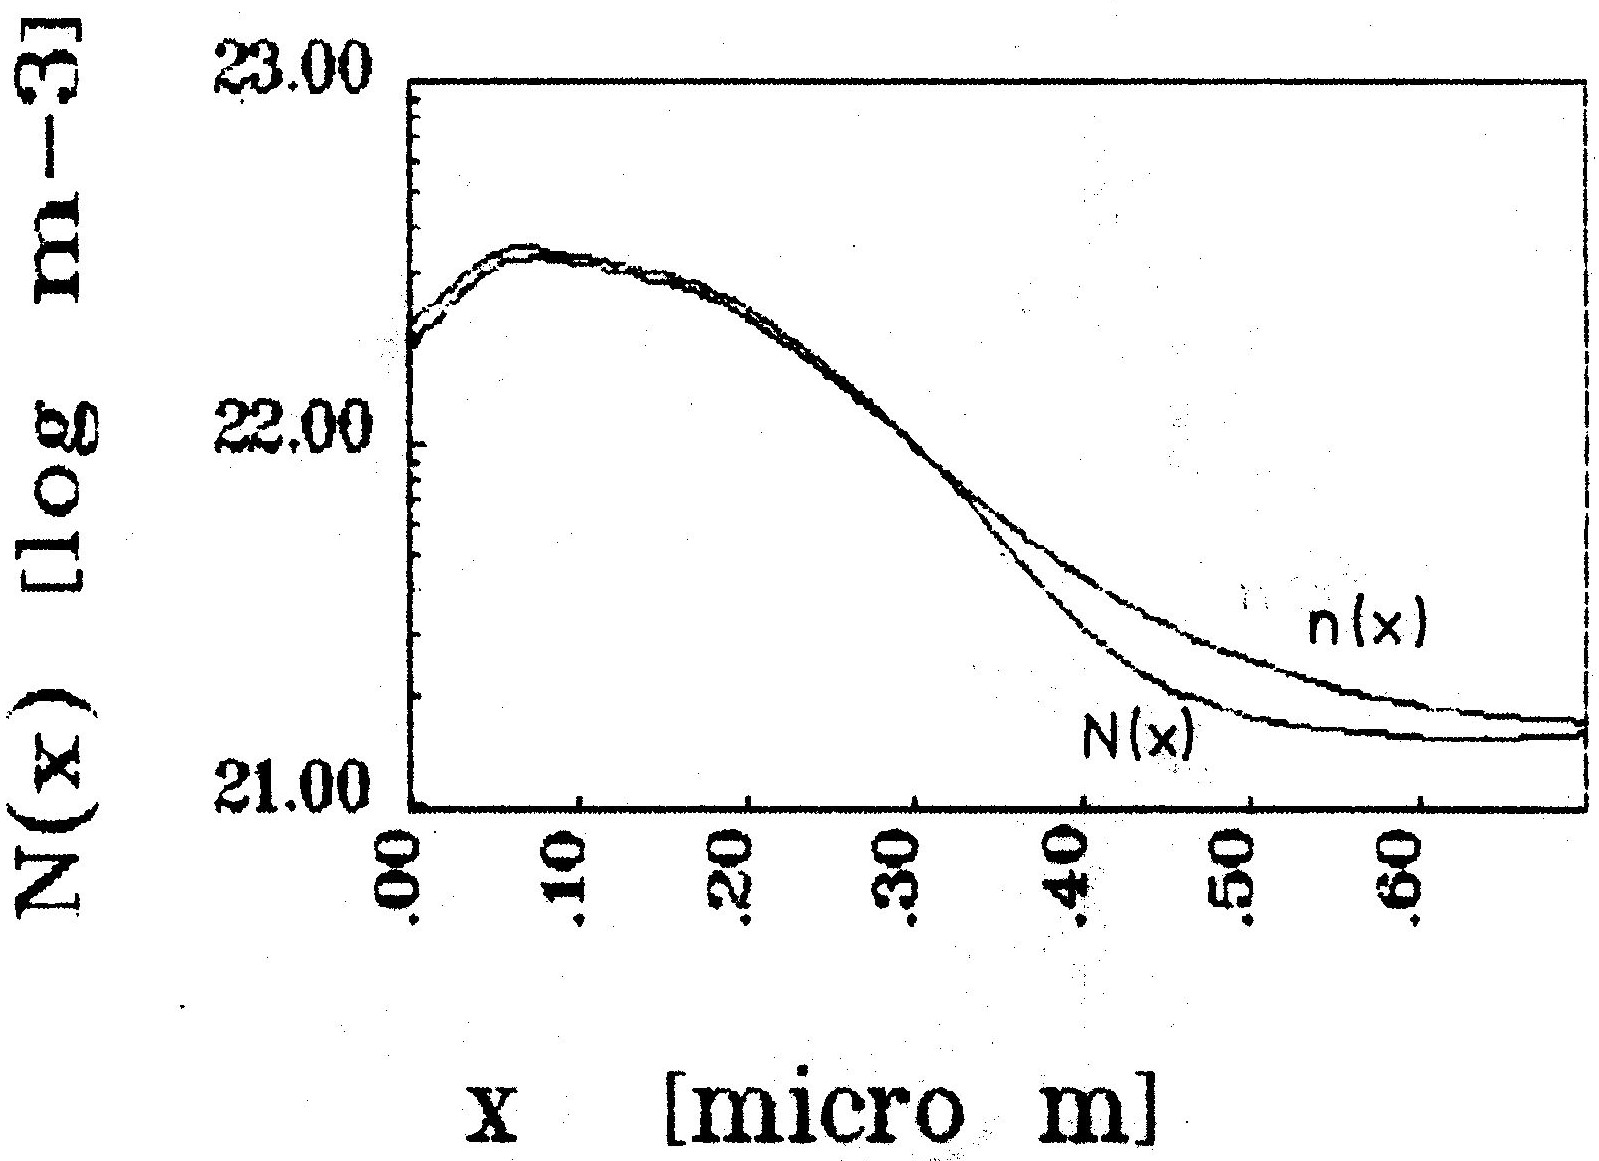
\includegraphics{Figures/fig-4-3.eps}
      \caption[Majority charge carrier concentration $n(x)$ determined
        from the depleted HF C-V dependence and the progression of the
        donating atoms $N (x)$ determined from the
        equation~\ref{eq:4.12}]{Concentration curve of major charge
        carriers $n (x)$ determined from the depleted HF C-V
        dependence and the path of the $N (x)$ donor atoms determined
        from equation~\ref{eq:4.12}.}\label{fig:4.3}
    \end{center}
  \end{minipage}
\end{figure}
% OBR23.BIT

\begin{equation}\label{eq:4.12}
  N(x) = n(x) - {\frac{kT\epsilon}{q^{2}} {\frac{d}{dx}} {\Bigg[\frac{1}{n(x)}\frac{dn(x)}{dx}\Bigg]}}
\end{equation}

Figure~\ref{fig:4.3} shows the curves of $n(x)$ and $N(x)$. In
equation~\ref{eq:4.12} the second derivative of $n(x)$ stands out,
which in the case of experimental values of $n(x)$ must be determined
numerically. Determining the derivative of an empirically obtained
functional dependence is a problem that can often be encountered when
processing measured data. In the basic numerical mathematics
courses~\cite{4.19} it is shown that differentiation amplifies the
noise of the processed data. In doing so, noise here generally refers
to the deviation of the processed data from its actual value that may
arise as a consequence of:

\begin{itemize}
\item physical phenomena
\item measurement instrument error
\item rounding in numerical processing.
\end{itemize}

\par That is, the frequency spectrum of the processed signal, obtained
by Fourier transformation, will contain components that must be
removed before (or during) the derivative calculation. V the following
we will talk about the approximation by polynomials, which most
commonly used, although the above statements also apply to other
classes of functions. If we use polynomial approximations to calculate
the derivative, the it is convenient to `smooth'~\cite{4.20} the
function values first. To suppress noise suppression, the frequency
properties of the numerical methods, which can be expressed in terms
of the transfer characteristics. This approach we can compare the
frequency properties of polynomial approximations and numerical
filters~\cite{4.21}.  The basic difference between the calculation of
the coefficients of digital filters and the coefficients of of
polynomial approximations is that in the first case we start from the
desired transmission characteristic and in the latter case are
coefficients are calculated from the least squares distance condition
of the processed data and the polynomial of a given degree. Hence
shortcomings of polynomial approximations:

\begin{itemize}
\item processed functional dependence may not be a polynomial, even
  though there is a polynomial that interpolates the measured values
\item frequency properties of the method are a secondary consequence
  of the degree of the polynomial used and the number of points
  through which the polynomial translates.
\end{itemize}

\par Because in our case we are processing functional dependencies
that are not polynomials in general, we have chosen to use numerical
filters. It may be mentioned here that for a successful application of
digital filters is important to design the critical frequency and
magnitude of the filter so that the filter does not affect the
amplitude of the signal in that part of the of the spectrum that
represents the useful signal. To determine the derivatives in
formula~\ref{eq:4.12}, we used a non-recursive differentiating
low-pass digital filter whose critical frequency is $f_{c}=0.1$ and
its size is $2n+1=11$.

\par It is known~\cite{4.18} that even the progression of $n(x)$,
determined from the measured C-V dependence, is subject to error if it
represents a non-homogeneous concentration profile. More precisely, it
can be argued~\cite{4.3} that the measured concentration $n(x)$
represents the average value of the concentration of the majority
carriers in a region of length on the order of a few $L_{DE}$. Then
the question is when else can one use the approximations described in
Sections~\ref{sec:4.1},~\ref{sec:4.2} and with what error. The results
of a computational experiment are described in~\cite{4.22}, where,
based on the experimentally determined profile $N(x)$, the the
theoretical depleted C-V curve and compared with the measured C-V
curve. If the experimental and theoretical C-V dependence agree, it
can be argued that $N(x)$ represents the true distribution of of the
dopants in the semiconductor.

\par Independently on~\cite{4.22} we have carried out an experiment
whose results we report. In Figures~\ref{fig:4.4} and~\ref{fig:4.5}
are show the $N(x)$ curves that were used in the calculation of the
theoretical C-V dependence. While solving the Poisson equation, we
also obtained the $n_{1}(x)$ major charge carrier concentration curve
for $V_{g}=0$, which differs from the concentration profile due to
diffusion of $N(x)$ atoms. From the theoretical C-V dependences, the
following theoretical C-V dependences were obtained using
approximations~\ref{eq:4.2} and~\ref{eq:4.6} the curves were
calculated $n_{2}(x)$.  We compared the $n(x)$ dependencies because
the matching of the concentration of the major charge carriers implies
a matching of the curve of the concentration of the donor atoms. As
can be seen in Figure~\ref{fig:4.4}, for this concentration profile,
the use of the capacitance method is appropriate, whereas in the case
of shown in Figure~\ref{fig:4.5}, a large difference between actual
$n_{1}(x)$ and the measured $n_{2}(x)$ profile.

\begin{figure}[h!]\centering
  \begin{minipage}[c]{\myfiguresize}
    \begin{center}
      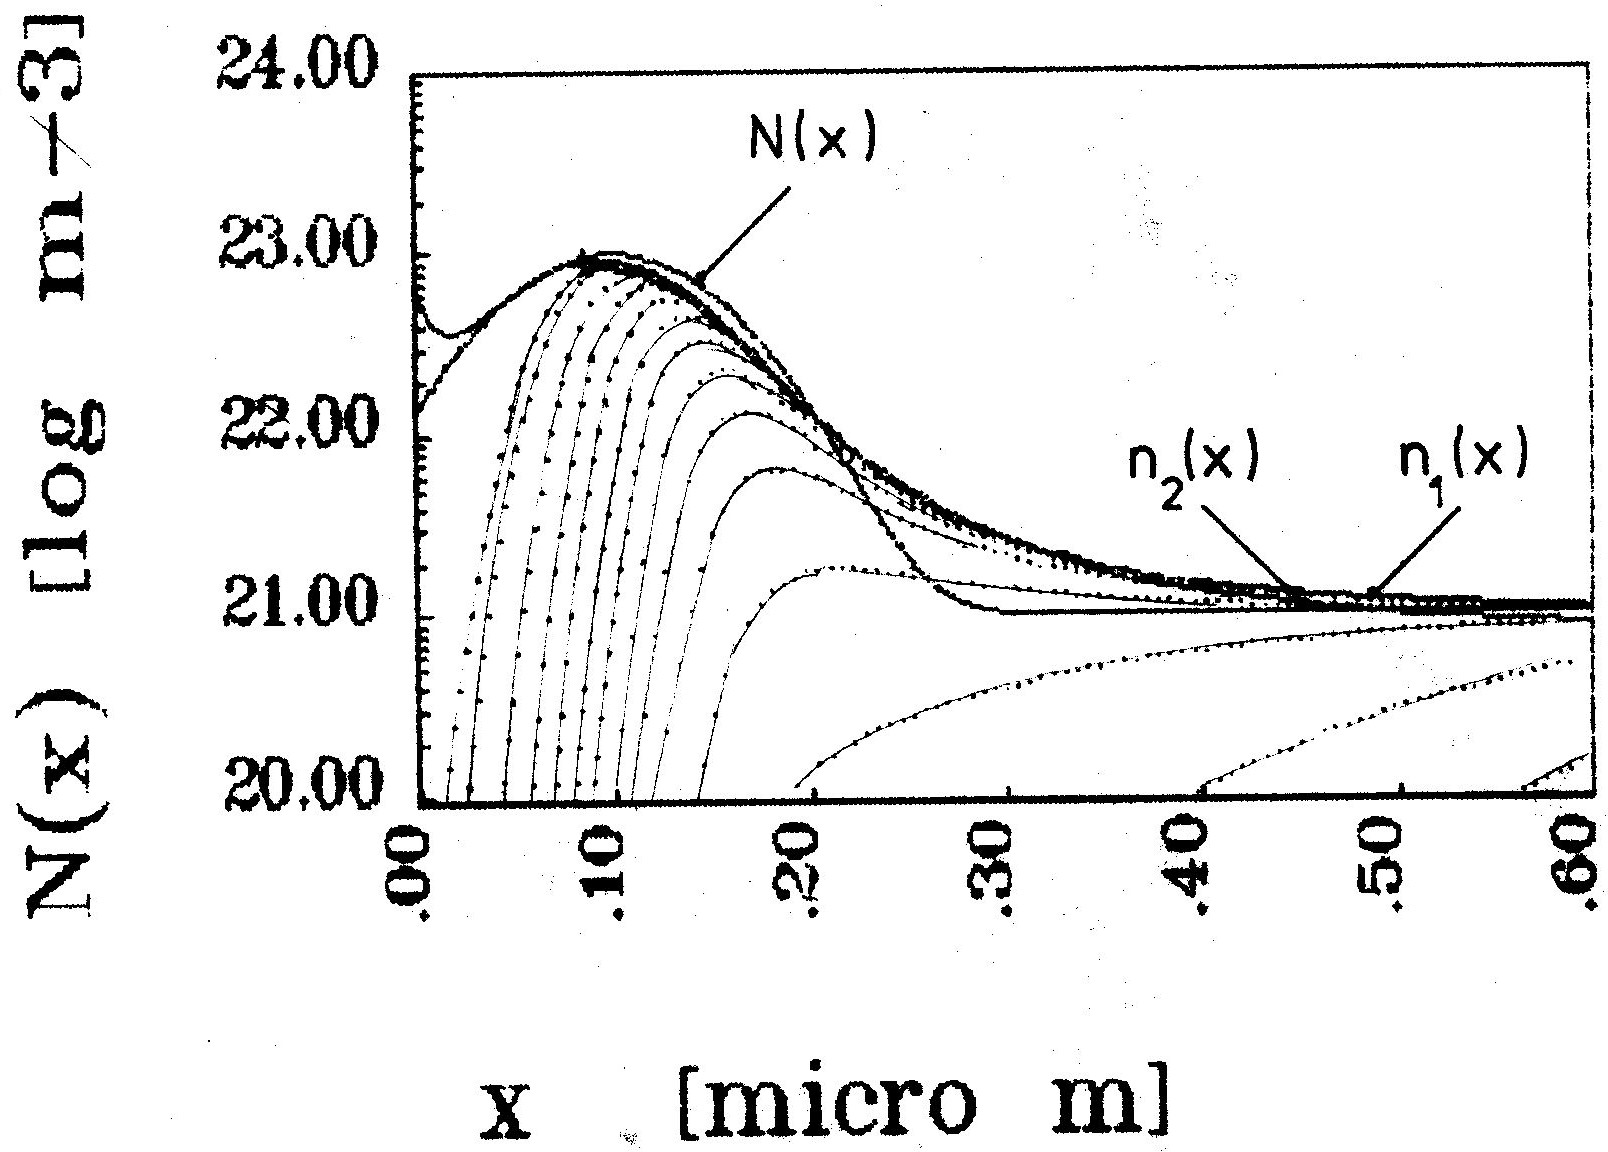
\includegraphics{Figures/fig-4-4.eps}
      \caption[Gaussian simulated impurity concentration
        distribution]{Admixture concentration profile $N(x)$ simulated
        by Gaussian distribution with parameters $R_{p}=0.1\mu m$,
        $\Delta R_{p}=0.05\mu m$, $N_{\max}=1.0\times 10^{23} m^{-3}$,
        $N_{bulk}=1.0\times10^{21}m^{-3}$; majority carrier
        progression charge $n_{1}(x)$ and the $n_{2}(x)$ curve
        obtained from the theoretical C-V dependence. The dotted lines
        show the depletion of the MOS structure.}\label{fig:4.4}
    \end{center}
  \end{minipage}
\end{figure}
% OBR24.BIT

\begin{figure}[h!]\centering
  \begin{minipage}[c]{\myfiguresize}
    \begin{center}
      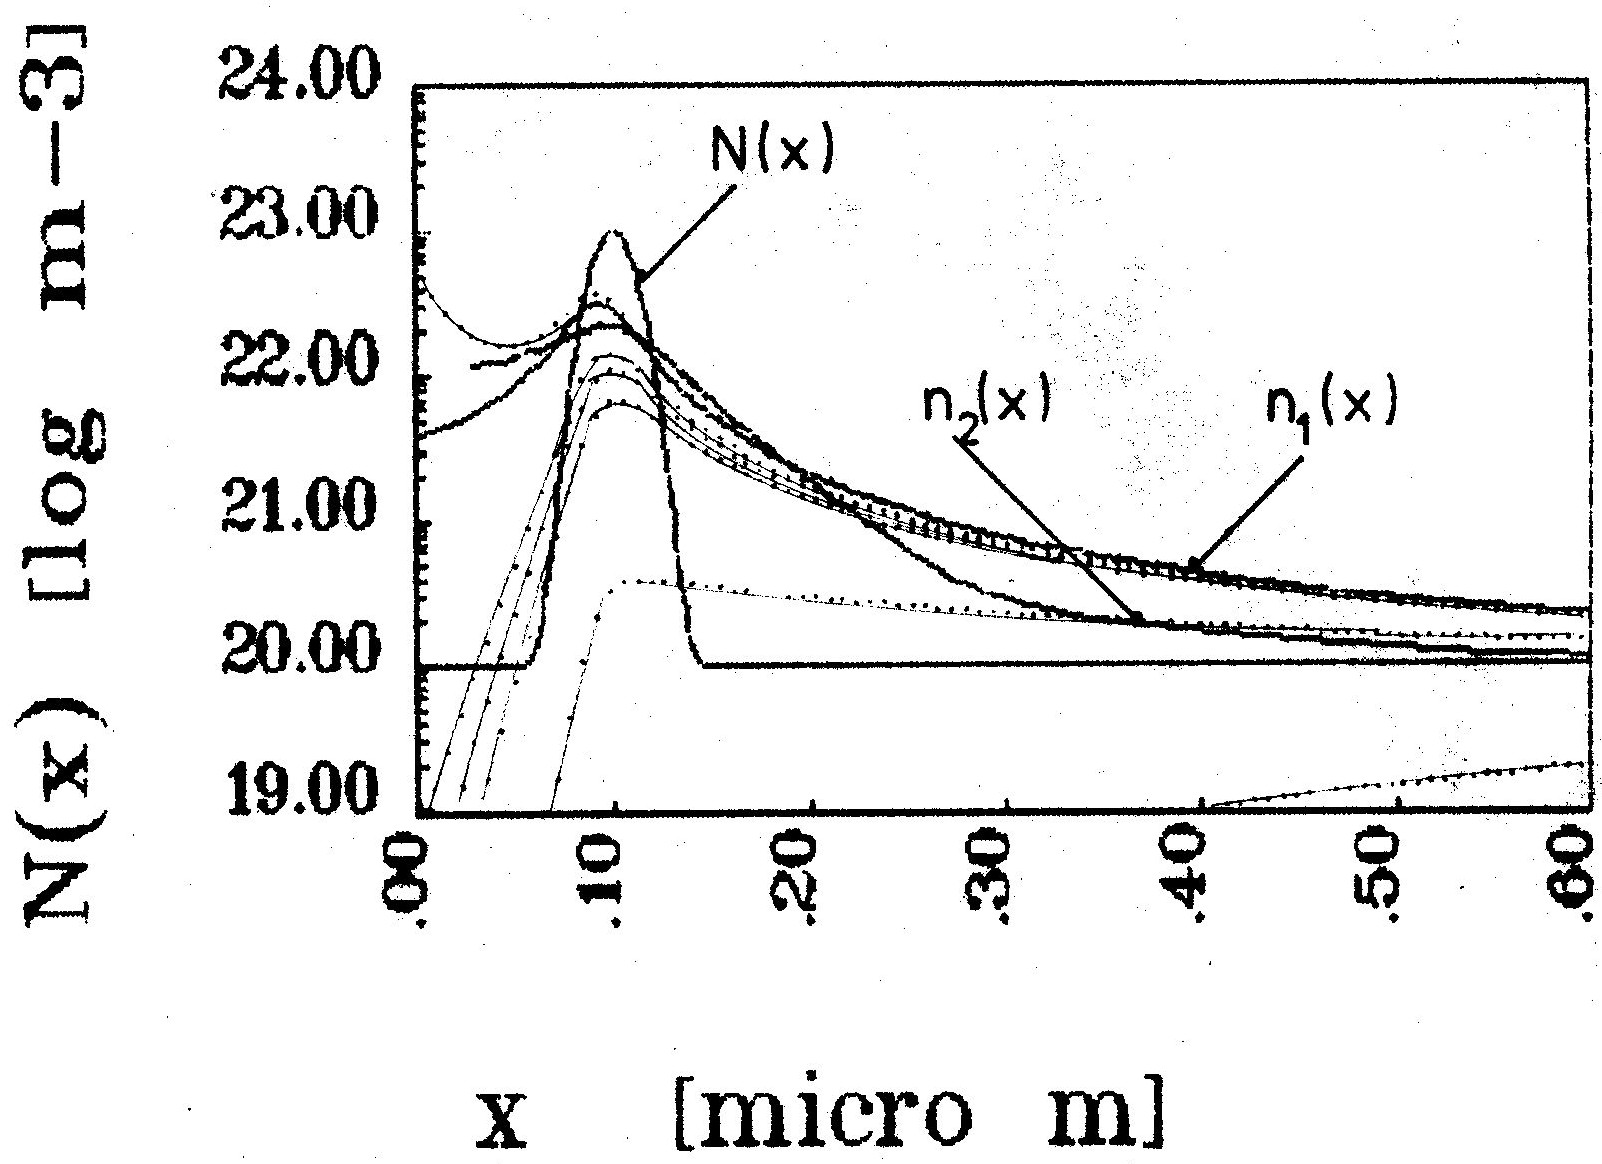
\includegraphics{Figures/fig-4-5.eps}
      \caption[Gaussian-simulated impurity concentration profile
        distribution]{Gaussian simulated $N(x)$ admixture
        concentration profile Gaussian distribution with parameters
        $R_{p}=0.1\mu m$, $\Delta R_{p}=0.01\mu m$,
        $N_{\max}=1.0\times10^{23}m^{-3}$,
        $N_{bulk}=1.0\times10^{21}m^{-3}$; majority carrier curve
        charge $n_{1}(x)$ and the $n_{2}(x)$ curve obtained from the
        theoretical C-V dependence. The dotted lines show the
        depletion of the MOS structure.}\label{fig:4.5}
    \end{center}
  \end{minipage}
\end{figure}
%OBR25.BIT

\par Further analysis of the approximations used in the calculation of
concentration profiles could focus on finding an exact bound validity
of these approximations, but from a systematic point of view it would
be to address this issue, it would be more efficient to take an
approach that to which the following remark refers.

\begin{minipage}[c]{\textwidth}
  \emph{NOTE.} Using capacitance measurements, it would be possible
  to determine $N(x)$ curve exactly without using the
  approximations given in previous articles.  In the work
  of~\cite{4.4} Appendix A it is indicated a procedure for calculating
  the electric potential in a semiconductor, which is a function of of
  the distance (from the semiconductor surface to the depth) and the
  gate voltage. Derivation of Poisson's equation~\ref{eq:1.2} by
  $V_{g}$ gives a third-order partial differential equation that
  accurately describes C-V dependence measurement experiment
  \begin{equation}\label{eq:4.13}
    \frac{\delta^{3}\varphi}{\delta x^{2}\delta V_{g}} = {\frac{1}{L_{D}^{2}}}\ {e^{\beta\varphi}}\ {\frac{\delta\varphi}{\delta V_{g}}}
  \end{equation}
  By solving it using appropriate boundary conditions, it would be
  possible to obtain a surface $\varphi(x,V_{g})$ from which to
  compute $N(x)$ only one line $\varphi(x)\rvert_{V_{g}}$
  \begin{equation}\label{eq:4.14}
    N(x) = N_{bulk}\ e^{\beta\varphi}-\frac{\epsilon}{q}\frac{\delta^{2}\varphi}{\delta x^{2}}
  \end{equation}
  (todo: check equation 4.14 in ref 4.4)
  The authors of paper~\cite{4.4} did not develop this method further
  for reasons the difficulty of quantifying the second derivative in
  the equation~\ref{eq:4.14}.
\end{minipage}

\section{Determination of $Si-SiO_{2}$ interface traps density.}\label{sec:4.2}

We characterize the quality of the $Si-SiO_{2}$ interface by the trap
density of the interface $(D_{it})$, which is a consequence of the
thermal oxidation mechanism of silicon, which produces a region of
non-stoichiometric composition. This density can be evaluated by the
following two procedures:

\begin{enumerate}
\item Comparison of measured high frequency C-V dependence
  $C_{mos}^{HF}(V_{g})$ and the measured low-frequency C-V dependence
  $C_{mos}^{LF}(V_{g})$. Evaluation of $D_{it}$ by comparison of the
  above dependencies is based on the assumption that the dependence
  $C_{mos}^{HF}(V_{g})$ is measured by a sufficiently high VF signal,
  which causes the capacitance to be unaffected by interface traps
  $Si-SiO_{2}$.
\item Comparison of the measured dependence of $C_{mos}^{LF}(V_{g})$
  and the theoretical low-frequency C-V dependence, which we denote
  $C_{mos}^{TLF}(V_{g})$.  In this case, based on the known
  concentration profile of the interfering impurities in the
  subsurface region of the semiconductor to calculate the dependence
  $C_{mos}^{TLF}(V_{g})$ by solving the Poisson equation.
\end{enumerate}

To evaluate $D_{it}$, we used both methods, the implementation of
which in we will detail in the following.

\subsection{Comparison of high and low frequency C-V dependence.}\label{sec:4.2.1}

In this case, we use the frequency dependence of the capacitance of
the MOS structure and $D_{it}$ is determined from the comparison of
$C_{mos}^{HF}(V_{g})$ and $C_{mos}^{LF}(V_{g})$. The necessary
theoretical basis can be found for example, in~\cite{I.1}.  To
determine $C_{mos}^{HF}(V_{g})$ and $C_{mos}^{LF}(V_{g})$, it is
convenient to use the Q-C method~\cite{3.4, 3.6, 3.7, 3.8}, which
allows simultaneous determination of both dependencies, but the use of
the standard methods for determining $C_{mos}^{HF}(V_{g})$ and
$C_{mos}^{LF}(V_{g})$ is also possible.

In figure~\ref{fig:4.6} the measured values of $C_{mos}^{HF}(V_{g})$
and surface potential $\varphi_{s}$ of the MOS structure, determined
by Q-C method. The curves are shown in Figure~\ref{fig:4.7}
$C_{mos}^{HF}(V_{g})$ and $C_{mos}^{LF}(V_{g})$, which we use for
calculate $D_{it}$ according to the following equation~\cite{4.15}

\begin{equation}\label{eq:4.15}
  D_{it} = {\cfrac{1}{q}} {\left[\cfrac{C_{mos}^{LF}}{1-\cfrac{C_{mos}^{LF}}{C_{ox}}}-\cfrac{C_{mos}^{HF}}{1-\cfrac{C_{mos}^{HF}}{C_{ox}}}\right]}
\end{equation}
% was (4.14) in origin

The position of the Fermi level in the forbidden band for the
calculated values $D_{it}$ are determined using the values of the
surface potential $\varphi_{s}$ and the distance of the Fermi surface
from the intrinsic Fermi surface $\varphi_{f}$. The surface potential
$\varphi_{s} (V_{g})$ is obtained either directly using the Q-C method
or by integration quasi-static C-V dependence using the Berglund
integral. In both both cases, we obtain the curves
$\varphi_{s} (V_{g})$, which are shifted in direction of the
$y$-axis. In the case of the Q-C method, this is a constant
$\varphi_{s0}$, which represents the surface potential if at the gate
of the MOS structure is not connected and in the case of the
quasi-static C-V method, the displacement represents the integration
constant. For both cases we can calculate the shift dependence
$\varphi_{s} (V_{g})$ using the procedure given in
Appendix~\ref{app:AppendixG}.

\newpage
\begin{figure}[h!]\centering
  \begin{minipage}[c]{\myfiguresize}
    \begin{center}
      % GNUPLOT: LaTeX picture with Postscript
\begingroup
  \makeatletter
  \providecommand\color[2][]{%
    \GenericError{(gnuplot) \space\space\space\@spaces}{%
      Package color not loaded in conjunction with
      terminal option `colourtext'%
    }{See the gnuplot documentation for explanation.%
    }{Either use 'blacktext' in gnuplot or load the package
      color.sty in LaTeX.}%
    \renewcommand\color[2][]{}%
  }%
  \providecommand\includegraphics[2][]{%
    \GenericError{(gnuplot) \space\space\space\@spaces}{%
      Package graphicx or graphics not loaded%
    }{See the gnuplot documentation for explanation.%
    }{The gnuplot epslatex terminal needs graphicx.sty or graphics.sty.}%
    \renewcommand\includegraphics[2][]{}%
  }%
  \providecommand\rotatebox[2]{#2}%
  \@ifundefined{ifGPcolor}{%
    \newif\ifGPcolor
    \GPcolortrue
  }{}%
  \@ifundefined{ifGPblacktext}{%
    \newif\ifGPblacktext
    \GPblacktexttrue
  }{}%
  % define a \g@addto@macro without @ in the name:
  \let\gplgaddtomacro\g@addto@macro
  % define empty templates for all commands taking text:
  \gdef\gplbacktext{}%
  \gdef\gplfronttext{}%
  \makeatother
  \ifGPblacktext
    % no textcolor at all
    \def\colorrgb#1{}%
    \def\colorgray#1{}%
  \else
    % gray or color?
    \ifGPcolor
      \def\colorrgb#1{\color[rgb]{#1}}%
      \def\colorgray#1{\color[gray]{#1}}%
      \expandafter\def\csname LTw\endcsname{\color{white}}%
      \expandafter\def\csname LTb\endcsname{\color{black}}%
      \expandafter\def\csname LTa\endcsname{\color{black}}%
      \expandafter\def\csname LT0\endcsname{\color[rgb]{1,0,0}}%
      \expandafter\def\csname LT1\endcsname{\color[rgb]{0,1,0}}%
      \expandafter\def\csname LT2\endcsname{\color[rgb]{0,0,1}}%
      \expandafter\def\csname LT3\endcsname{\color[rgb]{1,0,1}}%
      \expandafter\def\csname LT4\endcsname{\color[rgb]{0,1,1}}%
      \expandafter\def\csname LT5\endcsname{\color[rgb]{1,1,0}}%
      \expandafter\def\csname LT6\endcsname{\color[rgb]{0,0,0}}%
      \expandafter\def\csname LT7\endcsname{\color[rgb]{1,0.3,0}}%
      \expandafter\def\csname LT8\endcsname{\color[rgb]{0.5,0.5,0.5}}%
    \else
      % gray
      \def\colorrgb#1{\color{black}}%
      \def\colorgray#1{\color[gray]{#1}}%
      \expandafter\def\csname LTw\endcsname{\color{white}}%
      \expandafter\def\csname LTb\endcsname{\color{black}}%
      \expandafter\def\csname LTa\endcsname{\color{black}}%
      \expandafter\def\csname LT0\endcsname{\color{black}}%
      \expandafter\def\csname LT1\endcsname{\color{black}}%
      \expandafter\def\csname LT2\endcsname{\color{black}}%
      \expandafter\def\csname LT3\endcsname{\color{black}}%
      \expandafter\def\csname LT4\endcsname{\color{black}}%
      \expandafter\def\csname LT5\endcsname{\color{black}}%
      \expandafter\def\csname LT6\endcsname{\color{black}}%
      \expandafter\def\csname LT7\endcsname{\color{black}}%
      \expandafter\def\csname LT8\endcsname{\color{black}}%
    \fi
  \fi
    \setlength{\unitlength}{0.0500bp}%
    \ifx\gptboxheight\undefined%
      \newlength{\gptboxheight}%
      \newlength{\gptboxwidth}%
      \newsavebox{\gptboxtext}%
    \fi%
    \setlength{\fboxrule}{0.5pt}%
    \setlength{\fboxsep}{1pt}%
\begin{picture}(7920.00,5182.00)%
    \gplgaddtomacro\gplbacktext{%
      \csname LTb\endcsname%%
      \put(740,640){\makebox(0,0)[r]{\strut{}$0.5$}}%
      \put(740,1203){\makebox(0,0)[r]{\strut{}$0.6$}}%
      \put(740,1766){\makebox(0,0)[r]{\strut{}$0.7$}}%
      \put(740,2329){\makebox(0,0)[r]{\strut{}$0.8$}}%
      \put(740,2892){\makebox(0,0)[r]{\strut{}$0.9$}}%
      \put(740,3455){\makebox(0,0)[r]{\strut{}$1$}}%
      \put(740,4018){\makebox(0,0)[r]{\strut{}$1.1$}}%
      \put(740,4581){\makebox(0,0)[r]{\strut{}$1.2$}}%
      \put(860,440){\makebox(0,0){\strut{}$-2$}}%
      \put(1697,440){\makebox(0,0){\strut{}$-1$}}%
      \put(2535,440){\makebox(0,0){\strut{}$0$}}%
      \put(3372,440){\makebox(0,0){\strut{}$1$}}%
      \put(4210,440){\makebox(0,0){\strut{}$2$}}%
      \put(5047,440){\makebox(0,0){\strut{}$3$}}%
      \put(5884,440){\makebox(0,0){\strut{}$4$}}%
      \put(6722,440){\makebox(0,0){\strut{}$5$}}%
      \put(7559,440){\makebox(0,0){\strut{}$6$}}%
    }%
    \gplgaddtomacro\gplfronttext{%
      \csname LTb\endcsname%%
      \put(190,2610){\rotatebox{-270}{\makebox(0,0){\strut{}${C}/{C}_{ox}$ \qquad $(1-{\varphi}/{\varphi}_{norm})$}}}%
      \put(4209,140){\makebox(0,0){\strut{}Gate voltage ${V}_g$}}%
      \put(4209,4881){\makebox(0,0){\strut{}QC method}}%
      \csname LTb\endcsname%%
      \put(6142,1514){\makebox(0,0)[l]{\strut{}${C}_{mos}^{HF}$}}%
      \csname LTb\endcsname%%
      \put(6142,2293){\makebox(0,0)[l]{\strut{}${\varphi}_{s}^{HF}$}}%
    }%
    \gplbacktext
    \put(0,0){\includegraphics{/export/scratch/vbotka-thesis/Plot/Figures/fig-4-6-en}}%
    \gplfronttext
  \end{picture}%
\endgroup

      \caption[HF C-V $C_{mos}^{HF}(V_{g})$ and surface potential
        $\varphi_{s}(V_{g})$ of the MOS structure obtained using the
        Q-C method]{$C_{mos}^{HF}(V_{g})$ normalized to $C_{ox}$ and
        normalized surface potential $\varphi_{s}(V_{g})$ obtained by
        Q-C method. The surface potential is normalized by
        $1-{\varphi_{s}}/{\varphi_{norm}}$, where
        $\varphi_{norm}=3.33$.}\label{fig:4.6}
    \end{center}
  \end{minipage}
\end{figure}
% OBR15.BIT

\begin{figure}[h!]\centering
  \begin{minipage}[c]{\myfiguresize}
    \begin{center}
      % GNUPLOT: LaTeX picture with Postscript
\begingroup
  \makeatletter
  \providecommand\color[2][]{%
    \GenericError{(gnuplot) \space\space\space\@spaces}{%
      Package color not loaded in conjunction with
      terminal option `colourtext'%
    }{See the gnuplot documentation for explanation.%
    }{Either use 'blacktext' in gnuplot or load the package
      color.sty in LaTeX.}%
    \renewcommand\color[2][]{}%
  }%
  \providecommand\includegraphics[2][]{%
    \GenericError{(gnuplot) \space\space\space\@spaces}{%
      Package graphicx or graphics not loaded%
    }{See the gnuplot documentation for explanation.%
    }{The gnuplot epslatex terminal needs graphicx.sty or graphics.sty.}%
    \renewcommand\includegraphics[2][]{}%
  }%
  \providecommand\rotatebox[2]{#2}%
  \@ifundefined{ifGPcolor}{%
    \newif\ifGPcolor
    \GPcolortrue
  }{}%
  \@ifundefined{ifGPblacktext}{%
    \newif\ifGPblacktext
    \GPblacktexttrue
  }{}%
  % define a \g@addto@macro without @ in the name:
  \let\gplgaddtomacro\g@addto@macro
  % define empty templates for all commands taking text:
  \gdef\gplbacktext{}%
  \gdef\gplfronttext{}%
  \makeatother
  \ifGPblacktext
    % no textcolor at all
    \def\colorrgb#1{}%
    \def\colorgray#1{}%
  \else
    % gray or color?
    \ifGPcolor
      \def\colorrgb#1{\color[rgb]{#1}}%
      \def\colorgray#1{\color[gray]{#1}}%
      \expandafter\def\csname LTw\endcsname{\color{white}}%
      \expandafter\def\csname LTb\endcsname{\color{black}}%
      \expandafter\def\csname LTa\endcsname{\color{black}}%
      \expandafter\def\csname LT0\endcsname{\color[rgb]{1,0,0}}%
      \expandafter\def\csname LT1\endcsname{\color[rgb]{0,1,0}}%
      \expandafter\def\csname LT2\endcsname{\color[rgb]{0,0,1}}%
      \expandafter\def\csname LT3\endcsname{\color[rgb]{1,0,1}}%
      \expandafter\def\csname LT4\endcsname{\color[rgb]{0,1,1}}%
      \expandafter\def\csname LT5\endcsname{\color[rgb]{1,1,0}}%
      \expandafter\def\csname LT6\endcsname{\color[rgb]{0,0,0}}%
      \expandafter\def\csname LT7\endcsname{\color[rgb]{1,0.3,0}}%
      \expandafter\def\csname LT8\endcsname{\color[rgb]{0.5,0.5,0.5}}%
    \else
      % gray
      \def\colorrgb#1{\color{black}}%
      \def\colorgray#1{\color[gray]{#1}}%
      \expandafter\def\csname LTw\endcsname{\color{white}}%
      \expandafter\def\csname LTb\endcsname{\color{black}}%
      \expandafter\def\csname LTa\endcsname{\color{black}}%
      \expandafter\def\csname LT0\endcsname{\color{black}}%
      \expandafter\def\csname LT1\endcsname{\color{black}}%
      \expandafter\def\csname LT2\endcsname{\color{black}}%
      \expandafter\def\csname LT3\endcsname{\color{black}}%
      \expandafter\def\csname LT4\endcsname{\color{black}}%
      \expandafter\def\csname LT5\endcsname{\color{black}}%
      \expandafter\def\csname LT6\endcsname{\color{black}}%
      \expandafter\def\csname LT7\endcsname{\color{black}}%
      \expandafter\def\csname LT8\endcsname{\color{black}}%
    \fi
  \fi
    \setlength{\unitlength}{0.0500bp}%
    \ifx\gptboxheight\undefined%
      \newlength{\gptboxheight}%
      \newlength{\gptboxwidth}%
      \newsavebox{\gptboxtext}%
    \fi%
    \setlength{\fboxrule}{0.5pt}%
    \setlength{\fboxsep}{1pt}%
\begin{picture}(7920.00,5182.00)%
    \gplgaddtomacro\gplbacktext{%
      \csname LTb\endcsname%%
      \put(740,640){\makebox(0,0)[r]{\strut{}$0.5$}}%
      \put(740,1203){\makebox(0,0)[r]{\strut{}$0.6$}}%
      \put(740,1766){\makebox(0,0)[r]{\strut{}$0.7$}}%
      \put(740,2329){\makebox(0,0)[r]{\strut{}$0.8$}}%
      \put(740,2892){\makebox(0,0)[r]{\strut{}$0.9$}}%
      \put(740,3455){\makebox(0,0)[r]{\strut{}$1$}}%
      \put(740,4018){\makebox(0,0)[r]{\strut{}$1.1$}}%
      \put(740,4581){\makebox(0,0)[r]{\strut{}$1.2$}}%
      \put(860,440){\makebox(0,0){\strut{}$-2$}}%
      \put(1697,440){\makebox(0,0){\strut{}$-1$}}%
      \put(2535,440){\makebox(0,0){\strut{}$0$}}%
      \put(3372,440){\makebox(0,0){\strut{}$1$}}%
      \put(4210,440){\makebox(0,0){\strut{}$2$}}%
      \put(5047,440){\makebox(0,0){\strut{}$3$}}%
      \put(5884,440){\makebox(0,0){\strut{}$4$}}%
      \put(6722,440){\makebox(0,0){\strut{}$5$}}%
      \put(7559,440){\makebox(0,0){\strut{}$6$}}%
    }%
    \gplgaddtomacro\gplfronttext{%
      \csname LTb\endcsname%%
      \put(190,2610){\rotatebox{-270}{\makebox(0,0){\strut{}${C}/{C}_{ox}$}}}%
      \put(4209,140){\makebox(0,0){\strut{}Gate voltage ${V}_g$}}%
      \put(4209,4881){\makebox(0,0){\strut{}QC method}}%
      \csname LTb\endcsname%%
      \put(6142,1514){\makebox(0,0)[l]{\strut{}${C}_{mos}^{HF}$}}%
      \csname LTb\endcsname%%
      \put(6028,3400){\makebox(0,0)[l]{\strut{}${C}_{mos}^{LF}$}}%
    }%
    \gplbacktext
    \put(0,0){\includegraphics{/export/scratch/vbotka-thesis/Plot/Figures/fig-4-7-en}}%
    \gplfronttext
  \end{picture}%
\endgroup

      \caption[HF C-V $C_{mos}^{HF} (V_{g})$ and LF C-V dependence
        $C_{mos}^{LF} (V_{g})$ normalized to $C_{ox}$, obtained using
        the Q-C method]{HF C-V $C_{mos}^{HF} (V_{g})$ and LF C-V
        $C_{mos}^{LF} (V_{g})$ normalized to $C_{ox}$, obtained using
        the Q-C method.  LF C-V is calculated by deriving the surface
        potential (shown in Figure~\ref{fig:4.6}) according to the
        equation~\ref{eq:3.2}.}\label{fig:4.7}
    \end{center}
  \end{minipage}
\end{figure}
% OBR12.BIT

\newpage
\begin{figure}[h!]\centering
  \begin{minipage}[c]{\myfiguresize}
    \begin{center}
      % GNUPLOT: LaTeX picture with Postscript
\begingroup
  \makeatletter
  \providecommand\color[2][]{%
    \GenericError{(gnuplot) \space\space\space\@spaces}{%
      Package color not loaded in conjunction with
      terminal option `colourtext'%
    }{See the gnuplot documentation for explanation.%
    }{Either use 'blacktext' in gnuplot or load the package
      color.sty in LaTeX.}%
    \renewcommand\color[2][]{}%
  }%
  \providecommand\includegraphics[2][]{%
    \GenericError{(gnuplot) \space\space\space\@spaces}{%
      Package graphicx or graphics not loaded%
    }{See the gnuplot documentation for explanation.%
    }{The gnuplot epslatex terminal needs graphicx.sty or graphics.sty.}%
    \renewcommand\includegraphics[2][]{}%
  }%
  \providecommand\rotatebox[2]{#2}%
  \@ifundefined{ifGPcolor}{%
    \newif\ifGPcolor
    \GPcolortrue
  }{}%
  \@ifundefined{ifGPblacktext}{%
    \newif\ifGPblacktext
    \GPblacktexttrue
  }{}%
  % define a \g@addto@macro without @ in the name:
  \let\gplgaddtomacro\g@addto@macro
  % define empty templates for all commands taking text:
  \gdef\gplbacktext{}%
  \gdef\gplfronttext{}%
  \makeatother
  \ifGPblacktext
    % no textcolor at all
    \def\colorrgb#1{}%
    \def\colorgray#1{}%
  \else
    % gray or color?
    \ifGPcolor
      \def\colorrgb#1{\color[rgb]{#1}}%
      \def\colorgray#1{\color[gray]{#1}}%
      \expandafter\def\csname LTw\endcsname{\color{white}}%
      \expandafter\def\csname LTb\endcsname{\color{black}}%
      \expandafter\def\csname LTa\endcsname{\color{black}}%
      \expandafter\def\csname LT0\endcsname{\color[rgb]{1,0,0}}%
      \expandafter\def\csname LT1\endcsname{\color[rgb]{0,1,0}}%
      \expandafter\def\csname LT2\endcsname{\color[rgb]{0,0,1}}%
      \expandafter\def\csname LT3\endcsname{\color[rgb]{1,0,1}}%
      \expandafter\def\csname LT4\endcsname{\color[rgb]{0,1,1}}%
      \expandafter\def\csname LT5\endcsname{\color[rgb]{1,1,0}}%
      \expandafter\def\csname LT6\endcsname{\color[rgb]{0,0,0}}%
      \expandafter\def\csname LT7\endcsname{\color[rgb]{1,0.3,0}}%
      \expandafter\def\csname LT8\endcsname{\color[rgb]{0.5,0.5,0.5}}%
    \else
      % gray
      \def\colorrgb#1{\color{black}}%
      \def\colorgray#1{\color[gray]{#1}}%
      \expandafter\def\csname LTw\endcsname{\color{white}}%
      \expandafter\def\csname LTb\endcsname{\color{black}}%
      \expandafter\def\csname LTa\endcsname{\color{black}}%
      \expandafter\def\csname LT0\endcsname{\color{black}}%
      \expandafter\def\csname LT1\endcsname{\color{black}}%
      \expandafter\def\csname LT2\endcsname{\color{black}}%
      \expandafter\def\csname LT3\endcsname{\color{black}}%
      \expandafter\def\csname LT4\endcsname{\color{black}}%
      \expandafter\def\csname LT5\endcsname{\color{black}}%
      \expandafter\def\csname LT6\endcsname{\color{black}}%
      \expandafter\def\csname LT7\endcsname{\color{black}}%
      \expandafter\def\csname LT8\endcsname{\color{black}}%
    \fi
  \fi
    \setlength{\unitlength}{0.0500bp}%
    \ifx\gptboxheight\undefined%
      \newlength{\gptboxheight}%
      \newlength{\gptboxwidth}%
      \newsavebox{\gptboxtext}%
    \fi%
    \setlength{\fboxrule}{0.5pt}%
    \setlength{\fboxsep}{1pt}%
\begin{picture}(7920.00,5182.00)%
    \gplgaddtomacro\gplbacktext{%
      \csname LTb\endcsname%%
      \put(1100,640){\makebox(0,0)[r]{\strut{}$1\times10^{7}$}}%
      \put(1100,1625){\makebox(0,0)[r]{\strut{}$1\times10^{8}$}}%
      \put(1100,2611){\makebox(0,0)[r]{\strut{}$1\times10^{9}$}}%
      \put(1100,3596){\makebox(0,0)[r]{\strut{}$1\times10^{10}$}}%
      \put(1100,4581){\makebox(0,0)[r]{\strut{}$1\times10^{11}$}}%
      \put(1220,440){\makebox(0,0){\strut{}$0$}}%
      \put(2012,440){\makebox(0,0){\strut{}$0.05$}}%
      \put(2805,440){\makebox(0,0){\strut{}$0.1$}}%
      \put(3597,440){\makebox(0,0){\strut{}$0.15$}}%
      \put(4390,440){\makebox(0,0){\strut{}$0.2$}}%
      \put(5182,440){\makebox(0,0){\strut{}$0.25$}}%
      \put(5974,440){\makebox(0,0){\strut{}$0.3$}}%
      \put(6767,440){\makebox(0,0){\strut{}$0.35$}}%
      \put(7559,440){\makebox(0,0){\strut{}$0.4$}}%
    }%
    \gplgaddtomacro\gplfronttext{%
      \csname LTb\endcsname%%
      \put(190,2610){\rotatebox{-270}{\makebox(0,0){\strut{}$D_{it} [m^{-2}eV^{-1}]$}}}%
      \put(4389,140){\makebox(0,0){\strut{}$E_{c} - E [eV]$}}%
      \put(4389,4881){\makebox(0,0){\strut{}Trap density of interface $Si-SiO_{2}$}}%
    }%
    \gplbacktext
    \put(0,0){\includegraphics{/export/scratch/vbotka-thesis/Plot/Figures/fig-4-8-en}}%
    \gplfronttext
  \end{picture}%
\endgroup

      \caption[Dependence of $D_{it}$ on the position in the forbidden
        band of the semiconductor of a P-type semiconductor,
        determined from the comparison of $C_{mos}^{HF} (V_{g})$ and
        $C_{mos}^{LF} (V_{g})$]{The dependence of $D_{it}$ on the
        position in the forbidden band of a P-type semiconductor,
        determined from a comparison of $C_{mos}^{HF} (V_{g})$ and
        $C_{mos}^{LF} (V_{g})$, which are shown in
        Figure~\ref{fig:4.7}.}\label{fig:4.8}
    \end{center}
  \end{minipage}
\end{figure}
% OBR14.BIT

The value of the potential $\varphi_{f}$ is determined using the relation

\begin{equation}\label{eq:4.16}
  \varphi_{f} = \pm \frac{kT}{g} \ln{\frac{N_{b}}{n_{i}}}
\end{equation}

, where we assume knowledge of the substrate concentration
$N_{b}$. Potential $\varphi_{f}$ has a positive sign for a P-type
semiconductor. If for surface potential $\varphi_{s}$ we choose the
same orientation as for $\varphi_{f}$, the energy position of the
interface traps in the forbidden band is then determined using the
following relation

\begin{equation}\label{eq:4.17}
  E_{c} - E = 0.56 + \varphi_{s} + \varphi_{f}
\end{equation}

, where $0.56$ represents the distance of the lower edge of the
conductivity band $(E_{c})$ from the intrinsic Fermi level. Run
$D_{it}$ as a function of position in the forbidden band is shown
in Figure~\ref{fig:4.8}.

\newpage
\subsection{Comparison of experimental and theoretical quasi-static CV dependence.}\label{sec:4.2.2}

To calculate $D_{it}$ using this method, it is necessary to know the
curve the concentration profile of the interfering impurities in
the subsurface of the semiconductor $N(x)$ in order to calculate
$C_{mos}^{TLF}(V_{g})$. The theoretical dependence of
$C_{mos}^{TLF}(V_{g})$ of the MOS structure is calculated by the
numerical procedure described in Appendix~\ref{app:AppendixA}.  The
use of numerical methods in this case is necessary because the
analytical solution of the Poisson equation is not possible for the
general $N(x)$ concentration distribution.  For numerical solution of
the Poisson equation, we also calculate the dependence of the surface
potential on the gate voltage $\varphi_{s}(V_{g})$, which we use to
determine the position of the calculated interface trap density in the
forbidden band of the semiconductor.  Because during the numerical
calculation we do not take into account the breakdown charges in the
oxide layer and at the interface $Si-SiO_{2}$ both theoretically
determined dependencies $\varphi_{s}(V_{g})$ and
$C_{mos}^{TLF}(V_{g})$ will both be shifted with respect to the
measured quasi-static C-V dependence by the value of $V_{FB}$. To
shift the above dependencies we also need to know the value of
$V_{FB}$.

\par To calculate $D_{it}$ we therefore use $C_{mos}^{TLF}(V_{g})$,
which is not burdened by the trapping capacity of the $Si-SiO_{2}$
interface. At Figure~\ref{fig:4.9} the measured and theoretical LF C-V
dependence, which we use below to evaluate $D_{it}$ according to the
equation

\begin{equation}\label{eq:4.18}
  D_{it} = {\cfrac{1}{q}} {\left[\cfrac{C_{mos}^{LF}}{1-\cfrac{C_{mos}^{LF}}{C_{ox}}}-\cfrac{C_{mos}^{TLF}}{1-\cfrac{C_{mos}^{TLF}}{C_{ox}}}\right]}
\end{equation}

Figure~\ref{fig:4.10} shows the trap density of the interface as a
function of position in the forbidden band of the semiconductor
determined by in the above manner.  The disadvantage of the described
method lies in the time of calculating the theoretical low-frequency
C-V dependence. Although the comparison of theoretical and
experimental low-frequency C-V dependence gives values of $D_{it}$ in
a larger region of the forbidden band, for the evaluation of the areal
distribution $D_{it}$ on a silicon wafer, we have used the following
procedure due to time constraints described in section~\ref{sec:4.2.1}

\begin{figure}[h!]\centering
  \begin{minipage}[c]{\myfiguresize}
    \begin{center}
      % GNUPLOT: LaTeX picture with Postscript
\begingroup
  \makeatletter
  \providecommand\color[2][]{%
    \GenericError{(gnuplot) \space\space\space\@spaces}{%
      Package color not loaded in conjunction with
      terminal option `colourtext'%
    }{See the gnuplot documentation for explanation.%
    }{Either use 'blacktext' in gnuplot or load the package
      color.sty in LaTeX.}%
    \renewcommand\color[2][]{}%
  }%
  \providecommand\includegraphics[2][]{%
    \GenericError{(gnuplot) \space\space\space\@spaces}{%
      Package graphicx or graphics not loaded%
    }{See the gnuplot documentation for explanation.%
    }{The gnuplot epslatex terminal needs graphicx.sty or graphics.sty.}%
    \renewcommand\includegraphics[2][]{}%
  }%
  \providecommand\rotatebox[2]{#2}%
  \@ifundefined{ifGPcolor}{%
    \newif\ifGPcolor
    \GPcolortrue
  }{}%
  \@ifundefined{ifGPblacktext}{%
    \newif\ifGPblacktext
    \GPblacktexttrue
  }{}%
  % define a \g@addto@macro without @ in the name:
  \let\gplgaddtomacro\g@addto@macro
  % define empty templates for all commands taking text:
  \gdef\gplbacktext{}%
  \gdef\gplfronttext{}%
  \makeatother
  \ifGPblacktext
    % no textcolor at all
    \def\colorrgb#1{}%
    \def\colorgray#1{}%
  \else
    % gray or color?
    \ifGPcolor
      \def\colorrgb#1{\color[rgb]{#1}}%
      \def\colorgray#1{\color[gray]{#1}}%
      \expandafter\def\csname LTw\endcsname{\color{white}}%
      \expandafter\def\csname LTb\endcsname{\color{black}}%
      \expandafter\def\csname LTa\endcsname{\color{black}}%
      \expandafter\def\csname LT0\endcsname{\color[rgb]{1,0,0}}%
      \expandafter\def\csname LT1\endcsname{\color[rgb]{0,1,0}}%
      \expandafter\def\csname LT2\endcsname{\color[rgb]{0,0,1}}%
      \expandafter\def\csname LT3\endcsname{\color[rgb]{1,0,1}}%
      \expandafter\def\csname LT4\endcsname{\color[rgb]{0,1,1}}%
      \expandafter\def\csname LT5\endcsname{\color[rgb]{1,1,0}}%
      \expandafter\def\csname LT6\endcsname{\color[rgb]{0,0,0}}%
      \expandafter\def\csname LT7\endcsname{\color[rgb]{1,0.3,0}}%
      \expandafter\def\csname LT8\endcsname{\color[rgb]{0.5,0.5,0.5}}%
    \else
      % gray
      \def\colorrgb#1{\color{black}}%
      \def\colorgray#1{\color[gray]{#1}}%
      \expandafter\def\csname LTw\endcsname{\color{white}}%
      \expandafter\def\csname LTb\endcsname{\color{black}}%
      \expandafter\def\csname LTa\endcsname{\color{black}}%
      \expandafter\def\csname LT0\endcsname{\color{black}}%
      \expandafter\def\csname LT1\endcsname{\color{black}}%
      \expandafter\def\csname LT2\endcsname{\color{black}}%
      \expandafter\def\csname LT3\endcsname{\color{black}}%
      \expandafter\def\csname LT4\endcsname{\color{black}}%
      \expandafter\def\csname LT5\endcsname{\color{black}}%
      \expandafter\def\csname LT6\endcsname{\color{black}}%
      \expandafter\def\csname LT7\endcsname{\color{black}}%
      \expandafter\def\csname LT8\endcsname{\color{black}}%
    \fi
  \fi
    \setlength{\unitlength}{0.0500bp}%
    \ifx\gptboxheight\undefined%
      \newlength{\gptboxheight}%
      \newlength{\gptboxwidth}%
      \newsavebox{\gptboxtext}%
    \fi%
    \setlength{\fboxrule}{0.5pt}%
    \setlength{\fboxsep}{1pt}%
\begin{picture}(7920.00,5616.00)%
    \gplgaddtomacro\gplbacktext{%
      \csname LTb\endcsname%%
      \put(740,640){\makebox(0,0)[r]{\strut{}$0.5$}}%
      \put(740,1265){\makebox(0,0)[r]{\strut{}$0.6$}}%
      \put(740,1890){\makebox(0,0)[r]{\strut{}$0.7$}}%
      \put(740,2515){\makebox(0,0)[r]{\strut{}$0.8$}}%
      \put(740,3140){\makebox(0,0)[r]{\strut{}$0.9$}}%
      \put(740,3765){\makebox(0,0)[r]{\strut{}$1$}}%
      \put(740,4390){\makebox(0,0)[r]{\strut{}$1.1$}}%
      \put(740,5015){\makebox(0,0)[r]{\strut{}$1.2$}}%
      \put(860,440){\makebox(0,0){\strut{}$-2$}}%
      \put(1977,440){\makebox(0,0){\strut{}$-1$}}%
      \put(3093,440){\makebox(0,0){\strut{}$0$}}%
      \put(4210,440){\makebox(0,0){\strut{}$1$}}%
      \put(5326,440){\makebox(0,0){\strut{}$2$}}%
      \put(6443,440){\makebox(0,0){\strut{}$3$}}%
      \put(7559,440){\makebox(0,0){\strut{}$4$}}%
    }%
    \gplgaddtomacro\gplfronttext{%
      \csname LTb\endcsname%%
      \put(190,2827){\rotatebox{-270}{\makebox(0,0){\strut{}${C}/{C}_{ox}$}}}%
      \put(4209,140){\makebox(0,0){\strut{}Gate voltage ${V}_g$}}%
      \put(4209,5315){\makebox(0,0){\strut{}Comparison of measured and theoretical LF C-V}}%
      \csname LTb\endcsname%%
      \put(6780,3423){\makebox(0,0)[l]{\strut{}${C}_{mos}^{LF}$}}%
    }%
    \gplbacktext
    \put(0,0){\includegraphics{/export/scratch/vbotka-thesis/Plot/Figures/fig-4-9-en}}%
    \gplfronttext
  \end{picture}%
\endgroup

      \caption[Theoretical LF C-V dependence and measured LF C-V
        dependence]{Theoretical LF C-V dependence and measured LF C-V
        dependence MOS structures normalized to oxide
        capacitance.}\label{fig:4.9}
    \end{center}
  \end{minipage}
\end{figure}
% OBR11.BIT

\begin{figure}[h!]\centering
  \begin{minipage}[c]{\myfiguresize}
    \begin{center}
      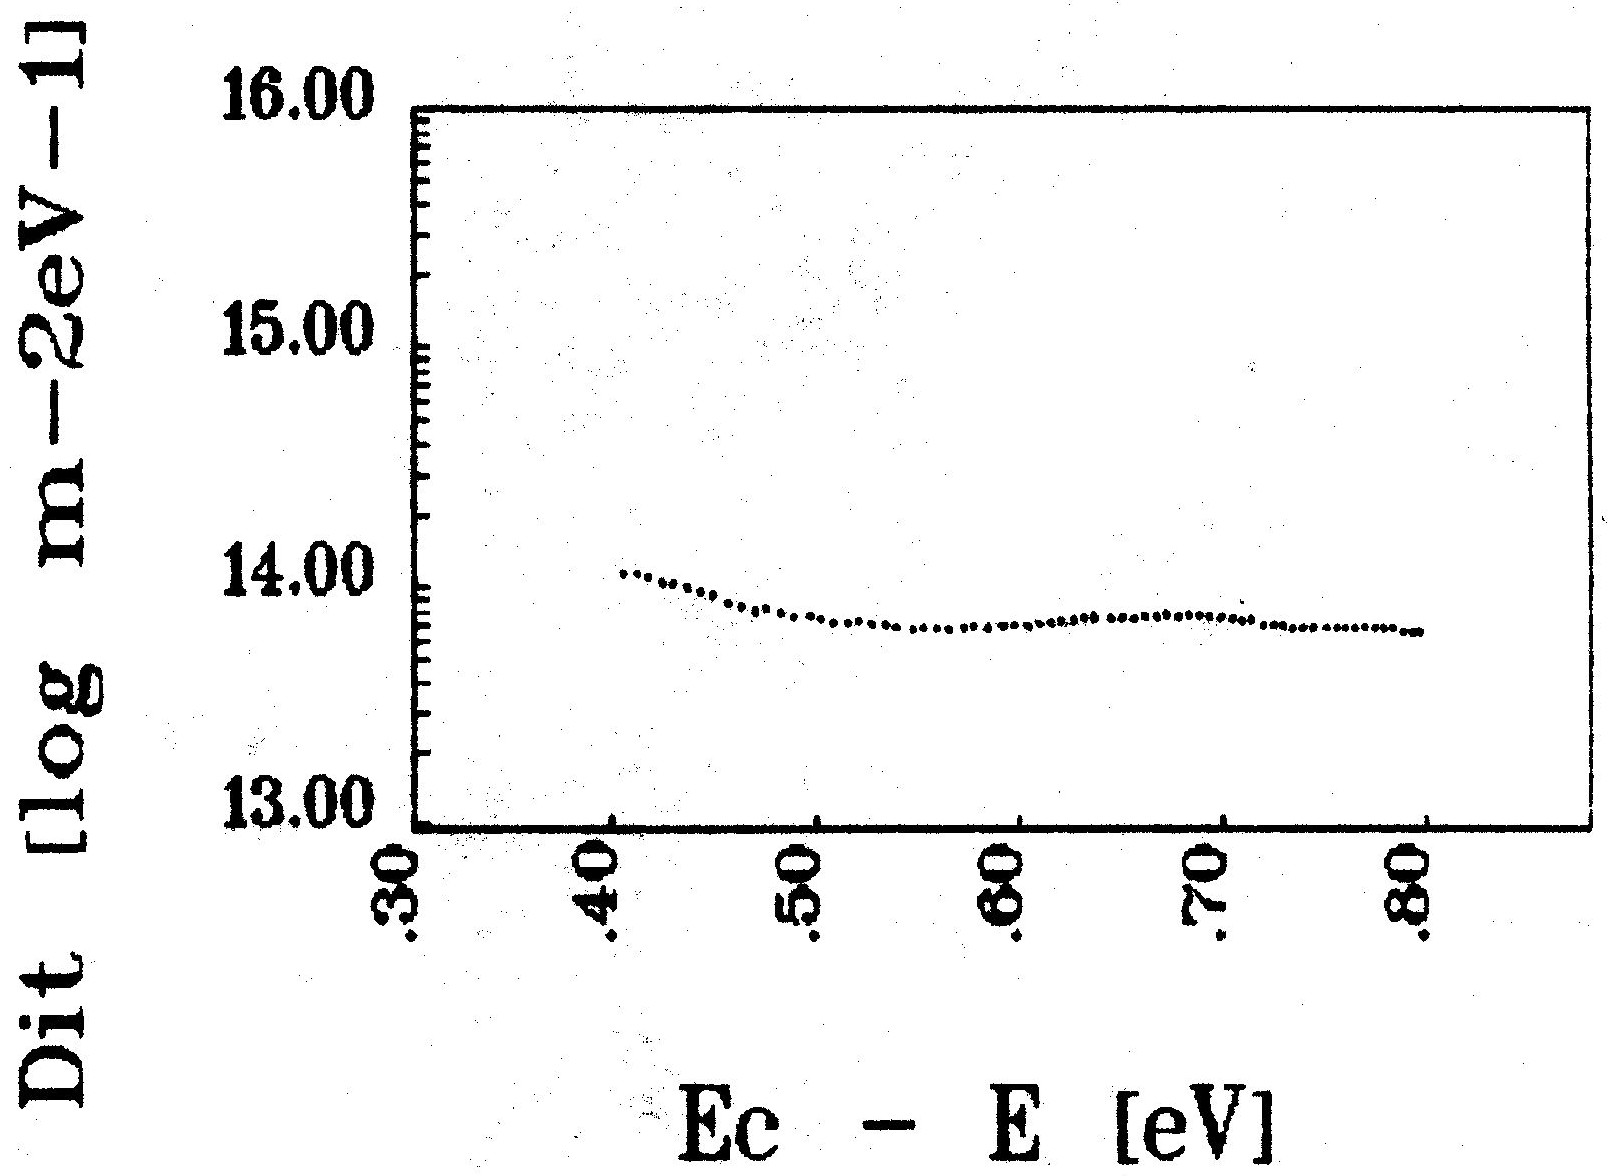
\includegraphics{Figures/fig-4-10.eps}
      \caption[Dependence of $D_{it}$ on the position in the forbidden
        band of the semiconductor determined from the comparison of
        $C_{mos}^{TLF}(V_{g})$ and $C_{mos}^{LF}(V_{g})$]{$D_{it}$
        dependence on the position in the forbidden band of a P-type
        semiconductor, determined from a comparison of
        $C_{mos}^{TLF}(V_{g})$ and $C_{mos}^{LF}(V_{g})$, which are
        shown in Figure~\ref{fig:4.9}.}\label{fig:4.10}
    \end{center}
  \end{minipage}
\end{figure}
% OBR13.BIT


\begin{thebibliography}{}
\bibitem[4.1]{4.1} Lehovec K.: Solid St\.  Electron.  27 (1984)
  s.1907.
\bibitem[4.2]{4.2} Wu Chung P., Douglas E.C., Mueller C.W.: IEEE
  Trans.\ on electron.\ dev. 22 (1975) s.319.
\bibitem[4.3]{4.3} Kroemer H., Chien W.: Solid St.\ Electron. 24
  (1981) s.655.
\bibitem[4.4]{4.4} Baccarani G., Rudan M., Maes H., Vandervorst W.,
  Van Overstraeten R.: Solid St\. Electron. 23 (1980) s. 65.
\bibitem[4.5]{4.5} Botka V., Csabay O., Artz P., Beyer A.: 3rd
  Scientific Conference EF SVŠT Elektrotechnika '90, EF SVŠT
  Bratislava, 1990 s.73.
\bibitem[4.6]{4.6} Kinder R.: Contribution to the investigation of
  concentrating profiles of implanted layers. Candidate's
  dissertation. EF SVŠT Bratislava 1984.
\bibitem[4.7]{4.7} Lin S.T., Reuter J.: Solid St.\ Electron. 26 (1983)
  s.343.
\bibitem[4.8]{4.8} Ziegler K., Klausmann E.: Solid St.\ Electron. 18
  (1975) s.189.
\bibitem[4.9]{4.9} Jindal R.P., Warner R.M. Jr.: IEEE Trans.\ on
  electron.\ dev. 28 (1981) s.348.
\bibitem[4.10]{4.10} Jindal R.P.: Solid St.\ Electron. 26 (1983)
  s.1005.
\bibitem[4.11]{4.11} Warner R.M. Jr., Jindal R.P.: Solid
  St.\ Electron. 26 (1983) s.335.
\bibitem[4.12]{4.12} Balland B., Remaki B., Marchand J.J.:
  J. Phys. E. Sci. Instrum. 21 (1988) s.559.
\bibitem[4.13]{4.13} Csabay O., Botka V.: 5th national conference
  Microelectronics 1989, House of Techniques CSVTS Bratislava, 1989
  p.58.
\bibitem[4.14]{4.14} Zsalkovics G.: Determination of the concentration
  profile of the implanted layer from capacitance
  measurements. Diploma thesis, Department Microelectronics, EF SVŠT,
  Bratislava 1988.
\bibitem[4.15]{4.15} Zohta Y.: Solid St.\ Electron. 17 (1974), s.1299.
\bibitem[4.16]{4.16} Kennedy O.P., Murley P.C., Kleinfelder W.: IBM
  J. Res. Dev. 12 (1968) p.399.
\bibitem[4.17]{4.17} Nishida V.: IEEE Trans. Electron. Dev. ED-26
  (1979) s.1081.
\bibitem[4.18]{4.18} Johnson W.C., Panousis P.T.: IEEE
  Trans. Electron. Dev. ED-18 (1971) s.965.
\bibitem[4.19]{4.19} Isaacson E., Keller H.B.: Analysis of numerical
  memethods.  John Wiley and Sons. New York.
\bibitem[4.20]{4.20} Vitásek E.: Numerické metody. SNTL, Praha 1987.
\bibitem[4.21]{4.21} Hamming R.W.: Digital filters. Prentice Hall.
\bibitem[4.22]{4.22} Beyer A., Tolonics J.: Physik der
  Halbleiteroberflache 17 (1986) s.91.
\end{thebibliography}
